\subsection{Drift Chambers (DC)}

\subsection{Geometry}

The DC geometry is implemented through the COATJAVA geometry service.
The service provides the Geant4 definitions that are read by the GEMC perl API to build the geometry database.

For each of the six sectors on the CLAS12 Forward Detector, there are three drift chambers: one in front of the torus,
one between the torus coils, and one after the torus.  These three chambers are referred to as different ``regions''.
The chambers are strung with the wires arranged in 12 internal layers.
Each layer is a generic G4Trapezoid, tilted by +6\mdeg or -6\mdeg depending if they are in the first or second
superlayer of a region.
The 12 layers in each region (6 per superlayer) are placed in a region mother volume made of air, see \F{dcGeometry}.
The layers are assigned the DC gas mixture: 90$\%$ Argon / 10$\%$ CO$_2$. Each layer is associated with the DC hit process routine.
The wire identification is performed in the Process ID routine.

\begin{figure}[h]
	\centering
	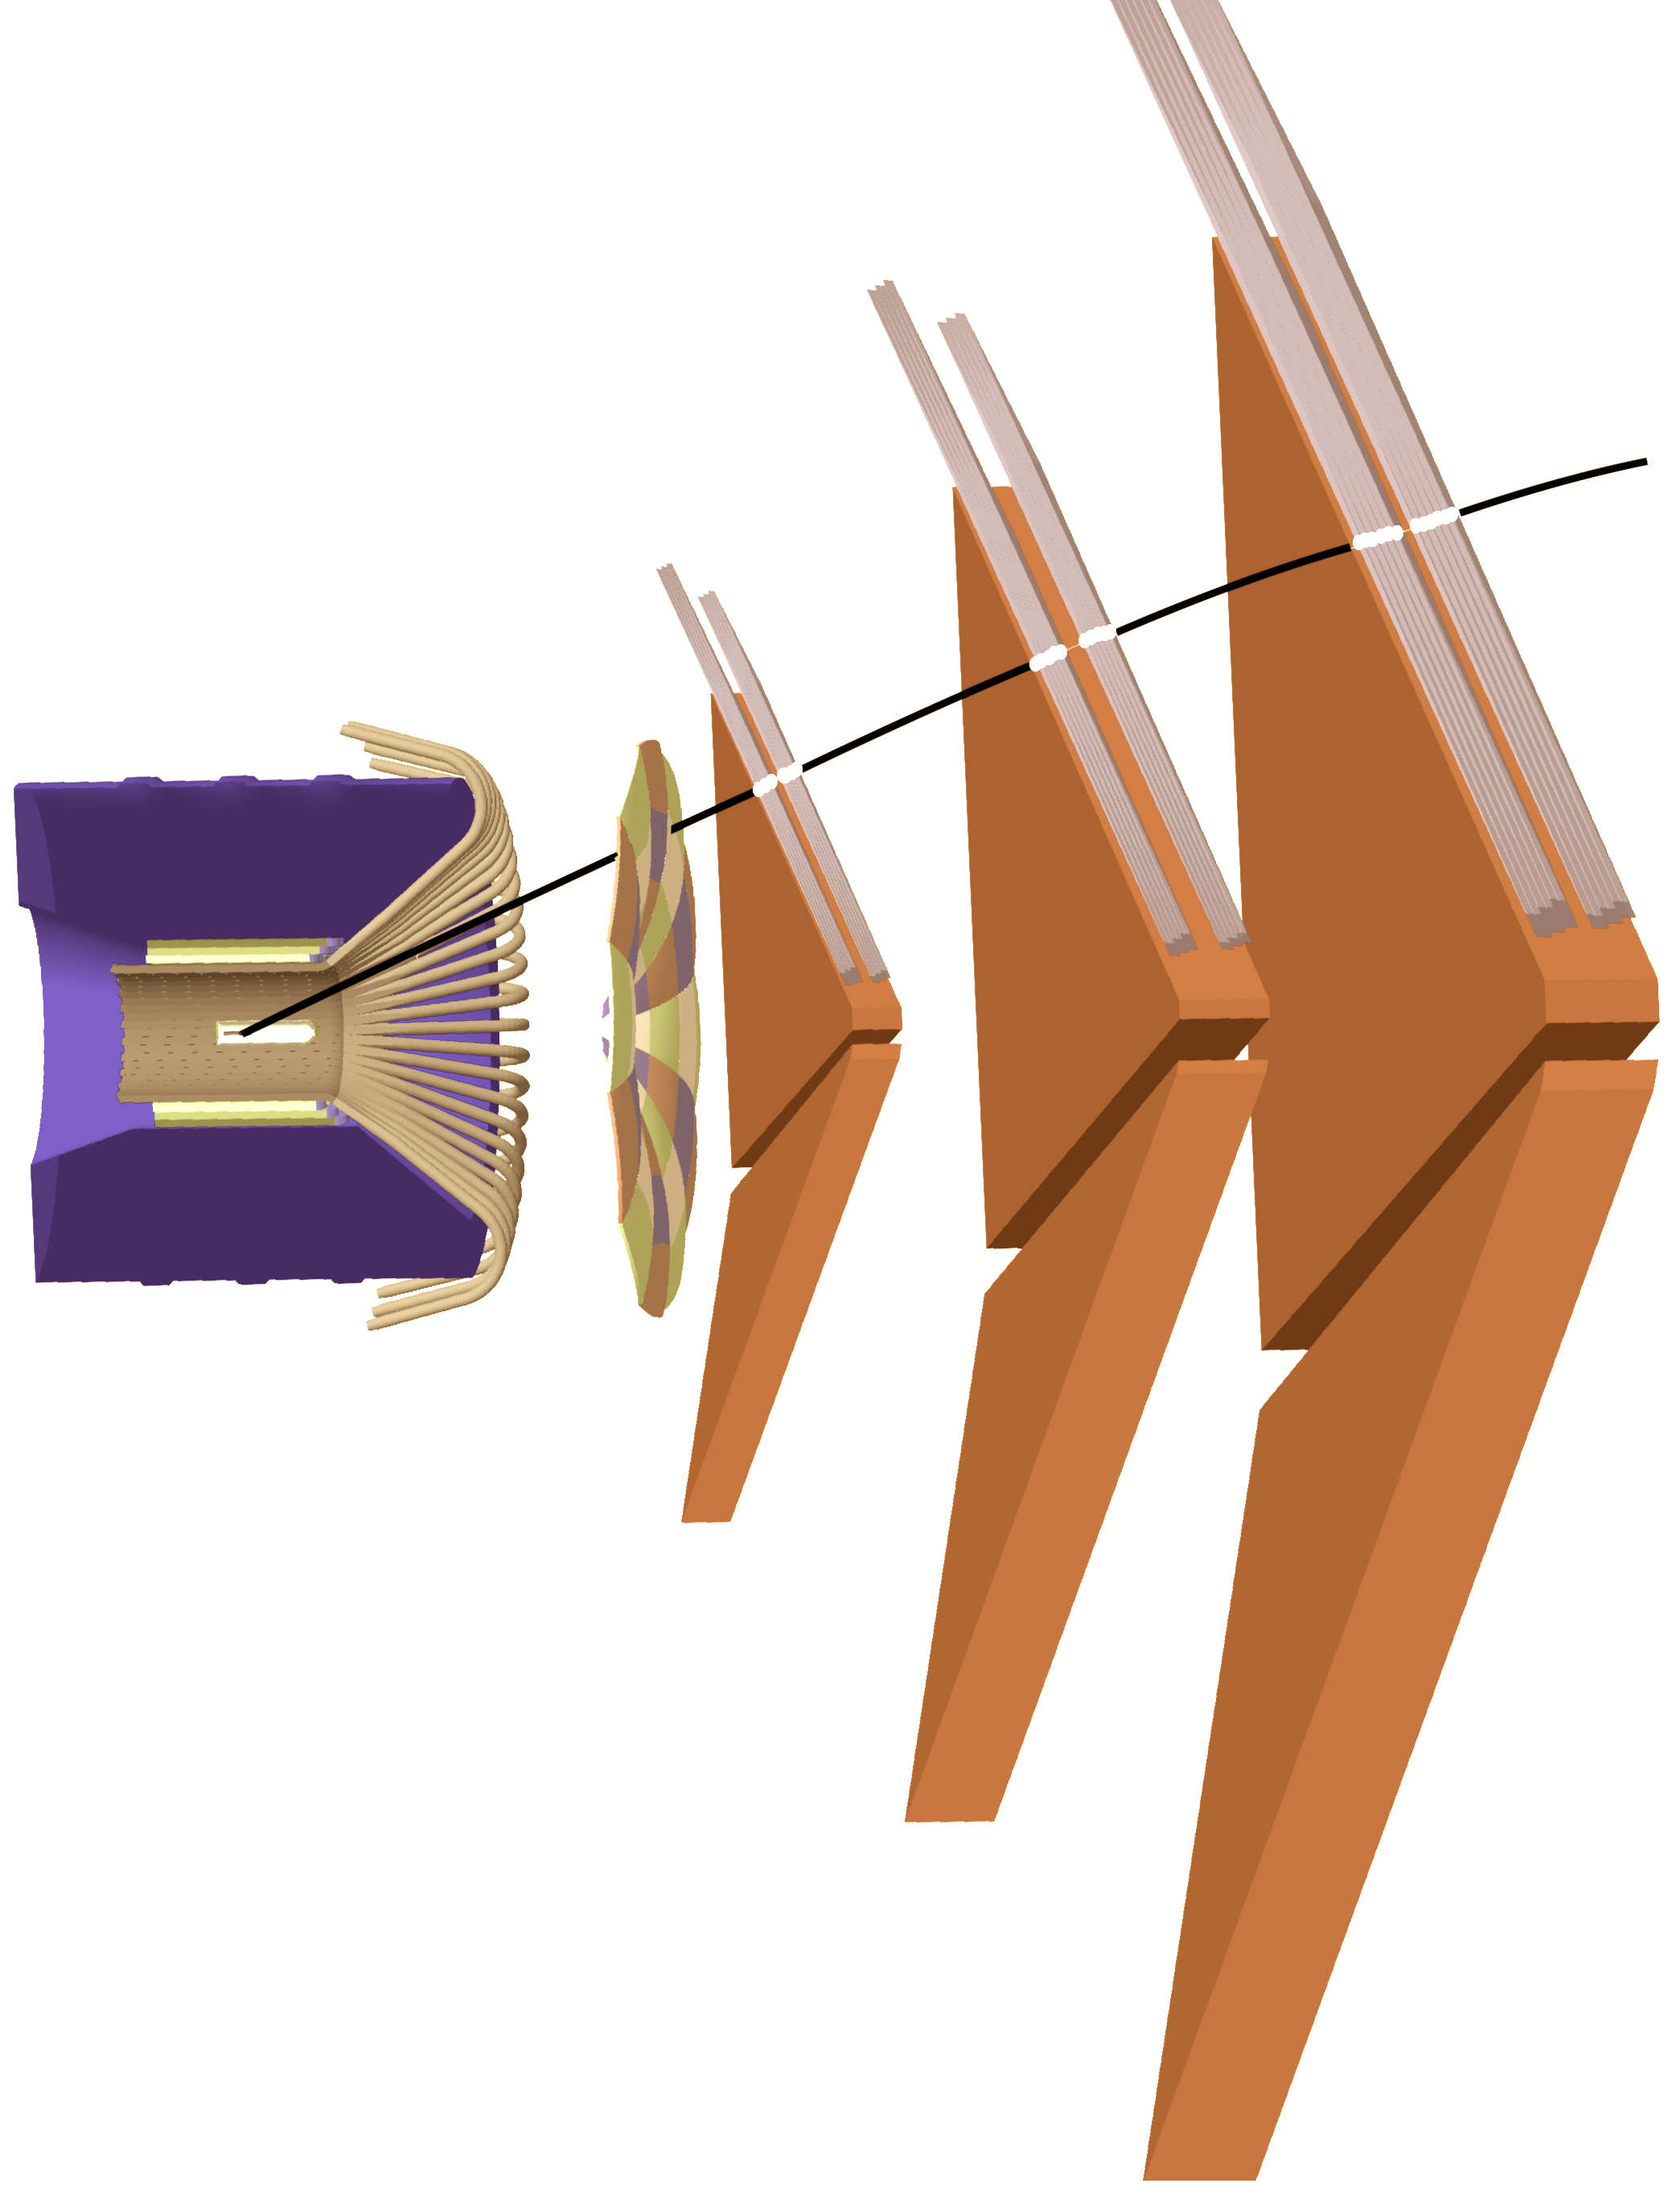
\includegraphics[width=0.99\columnwidth,keepaspectratio]{img/dcGeometry.png}
%	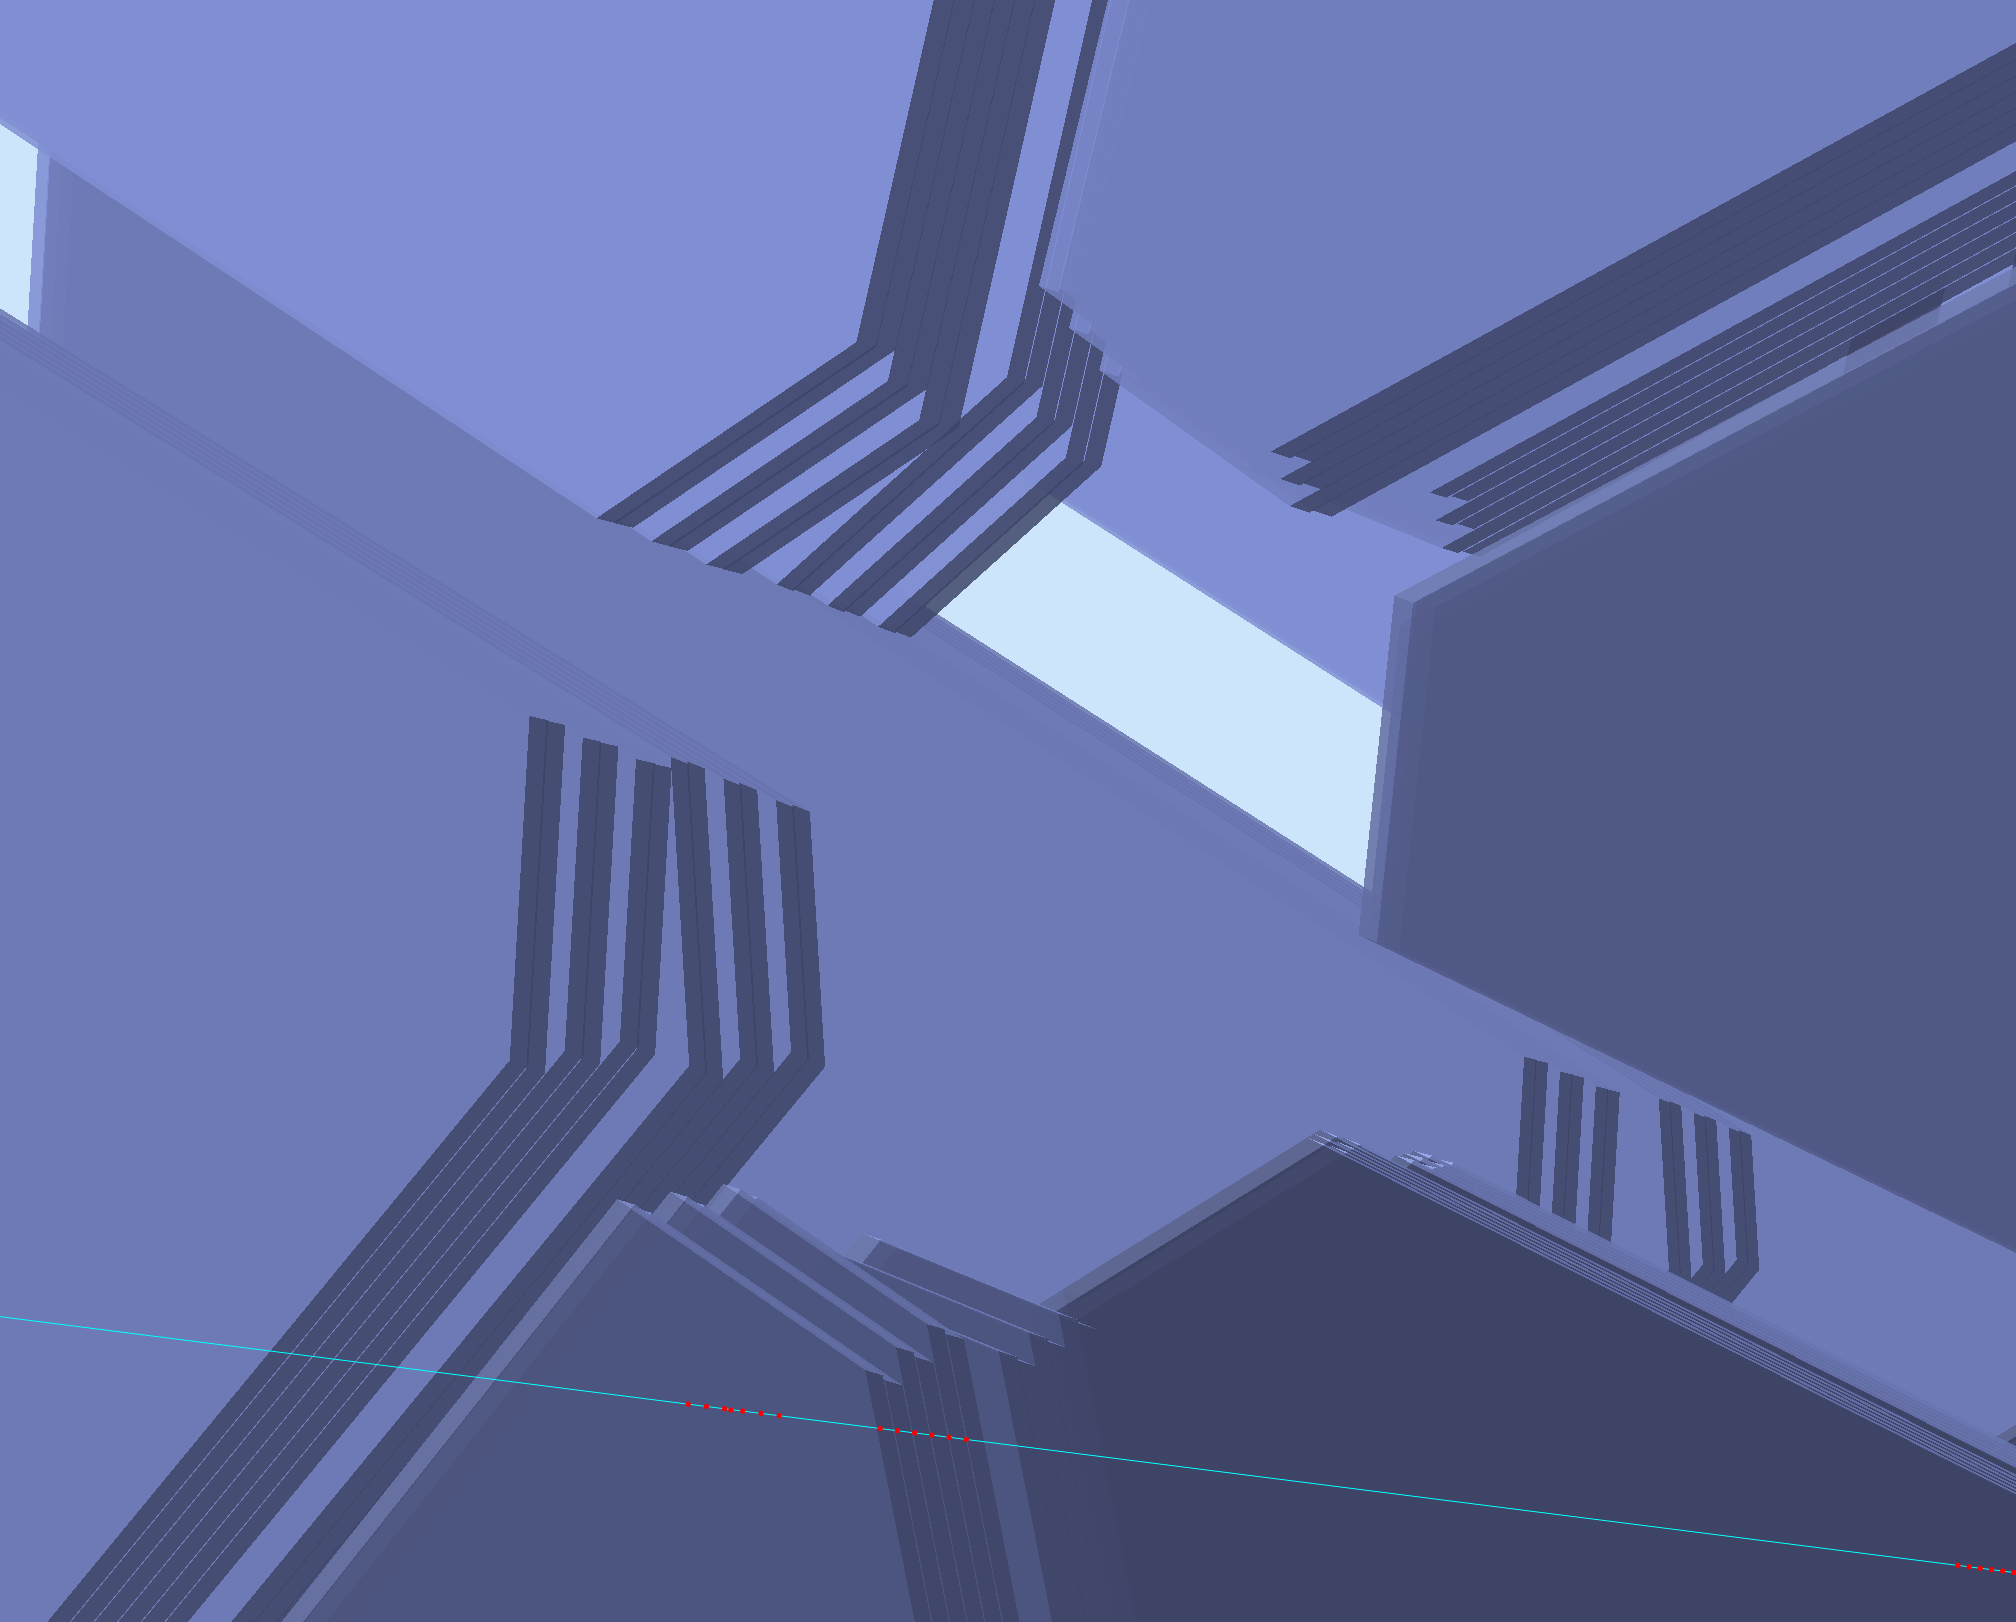
\includegraphics[width=0.99\columnwidth,keepaspectratio]{img/dcDetail.png}
	\caption{The GEMC implementation of the DC geometry. The solenoid volume and HTCC are also visible.
             Geant4 trapezoids are the mother volumes corresponding to DC regions 1, 2, and 3. The track is negative pion,
			 hitting the various layers inside each region. The hit are indicated by the black markers. Due to the high DC
             efficiency most tracks produce at least one hit each layer (12 hits / region).
             The wire inefficencies are incorporated in the simulation parameters, so wires can ``miss'' a hit just as in the experimental data.}
	\label{fig:dcGeometry}
\end{figure}

The Github location of the GEMC perl API script is \url{https://github.com/gemc/detectors/tree/master/clas12/dc}.
The java geometry service is at
\url{https://github.com/JeffersonLab/clas12-offline-software/blob/development/common-tools/clas-jcsg/src/main/java/org/jlab/detector/geant4/v2/DCGeant4Factory.java}.

\subsection{Process ID}
At each Geant4 step, the local vertical position $y$ in the DC layer volume is computed. Knowing the distance
between each wire $\delta Y$ (given by the total height of the trapezoid divided by the number of wires, $112$),
The wire sagging due to gravity and mechanical deflections of the wire endplates due to the tension load is not taken into account.
The wire ID is given by $n_i = y / \delta y$.

\subsection{Digitization}

First, the distance of closest approach ($DOCA$) is extrapolated for the hit.
At each Geant4 step, the distance of the track from the wire is calculated.
The $DOCA$ is extracted among the points with energy deposited larger than 50 eV,
for which the sum of the step time + $DOCA$/DV (where DV is the drift velocity) is minimal.

An initial time $T_i$ is calculated with a time to distance function that is the inverse of
what is determined from calibration and used in reconstruction to go from TDC to $DOCA$.
The function takes into account:

\begin{itemize}
	\item the distance from the wire, in cm;
	\item the cell size in superlayer;
	\item the polar angle of the track;
	\item magnitude of field in Tesla.
\end{itemize}

A time walk correction function $T_w$ is applied to $T_i$ that includes discrete ionization effects based on the following input:

\begin{itemize}
	\item the distance from the wire, in cm;
	\item the cell size in superlayer;
	\item an adjustable factor (in mm) times $\beta^2$ of the particle (the square of the particle speed).
	      The factor is adjusted according to data at small distances from the wire;
	\item the velocity of the particle.
\end{itemize}

The resulting $T_w$ is then used in a Landau-function to mimic the detector response function.

An intrinsic random time walk correction $\sigma_{TW}$ due to multiple scattering is calculated and the time is smeared with
a Gaussian function using $\sigma_{TW}$ as the resolution.
A random number is thrown (between 0 and 1) and if it is above the efficiency function, calculated based on $DOCA$, the hit is rejected.
Finally, the timing is smeared using the calibrated residual versus $DOCA$ function, see \F{dcResolution}.

\begin{figure}
	\centering
	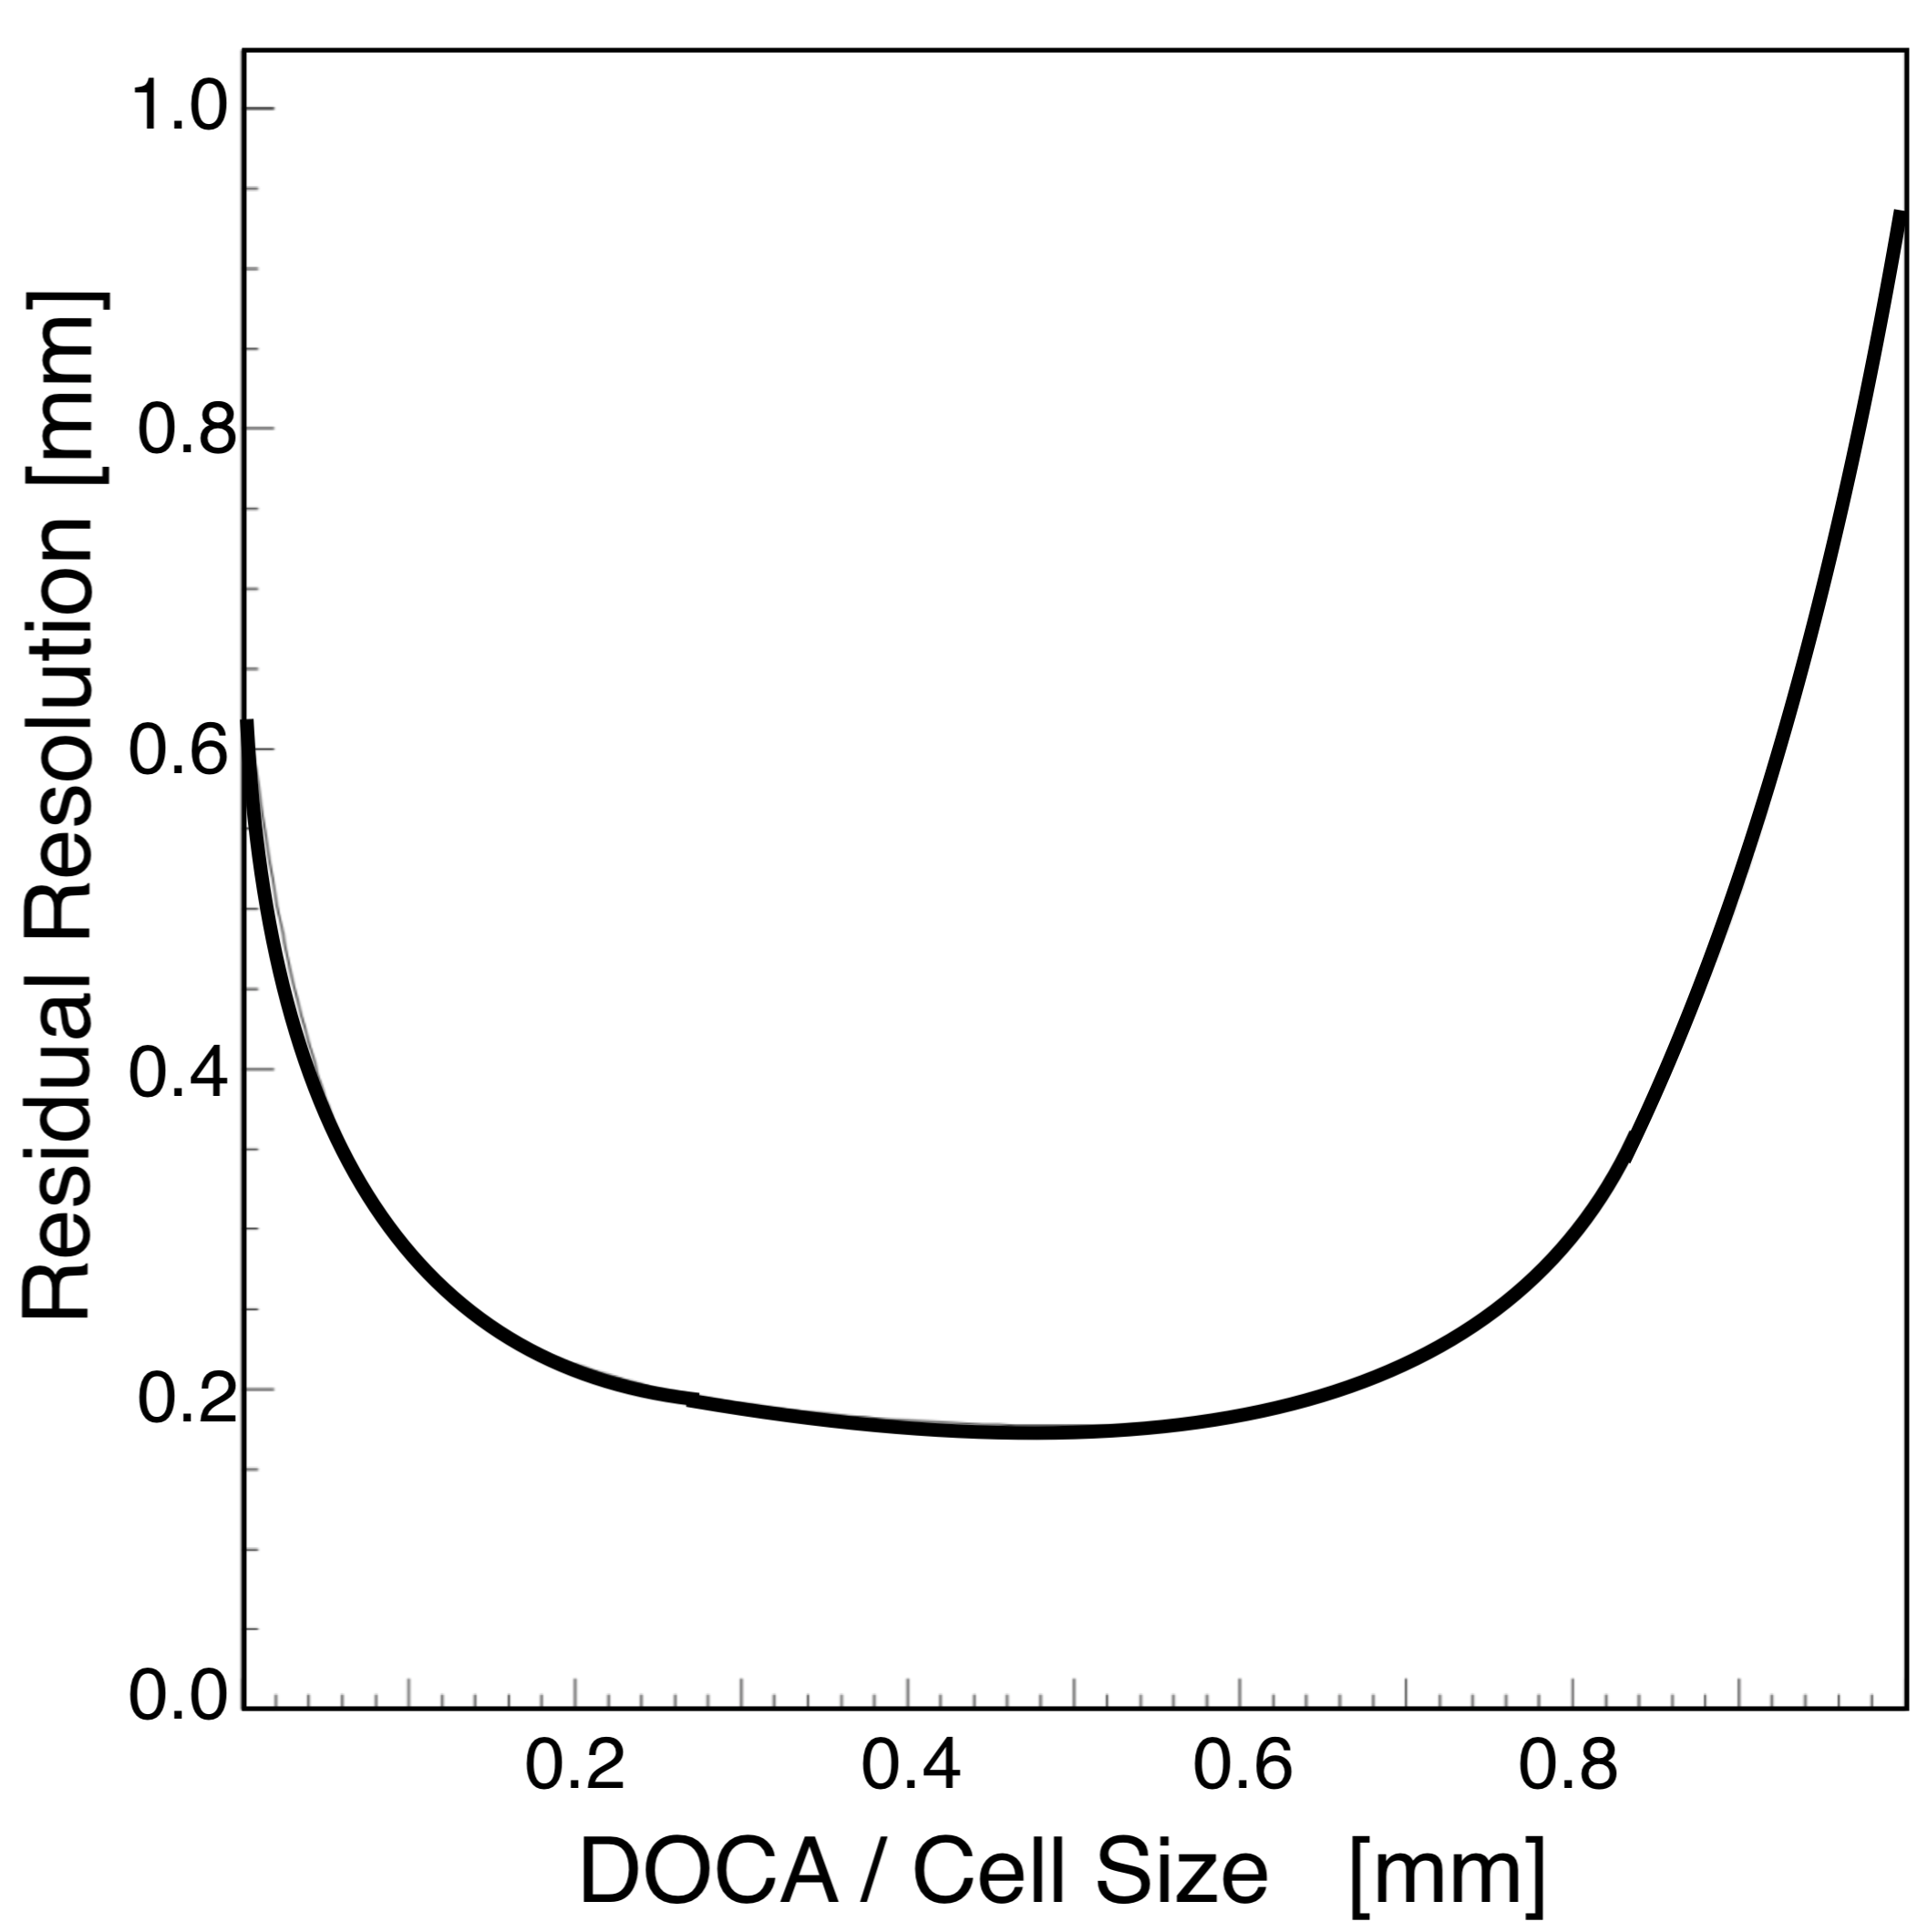
\includegraphics[width=0.99\columnwidth,keepaspectratio]{img/dcResolution.png}
	\caption{The fit to the data resolution provides parameters that are put in the CCDB database and read by the digitization routine at simulation run time.}
	\label{fig:dcResolution}
\end{figure}

The digitized output bank variables are summarized in Table \ref{tab:dcBank}.

\begin{table}[h]
	\begin{center}
		\begin{tabular}{| c | c | c |}
			\hline \hline
			Variable   & Description \\
			\hline
               sector  &                    sector index   \\
                layer  &                     layer index   \\
                 wire  &                      wire index   \\
                  tdc  &                       tdc value   \\
                   LR  &            Left/Right ambiguity   \\
                 doca  & 2D distance of closest approach   \\
                sdoca  &                    smeared doca   \\
                 time  &           doca / drift velocity   \\
                stime  &          sdoca / drift velocity   \\
			\hline \hline
		\end{tabular}
	\end{center}
	\caption{The digitized DC bank.}\label{tab:dcBank}
\end{table}


The simulation time window of the DC is set to 500 ns: all geant4 steps within the same cell and time window will be collected on one hit.
The actual electronic time window is set to 250, 500 and 750 ns for Regions 1, 2, and 3 respectively. This must be taken into account
The DC hit process routine location in git is \url{https://github.com/gemc/source/blob/master/hitprocess/clas12/dc_hitprocess.cc}


\subsubsection{Background Rates}

A detailed study of the background rates coming from beam interacting with the target was done to ensure that the DC occupancy stays
within limits that do not affect the reconstruction efficiency, typically below $5\%$.

Given the nominal operating luminosity $L=10^{35}$ cm$^{-2}$s$^{-1}$, and the liquid-hydrogen target length of 5 cm, the beam electron rate
is R=4.7 $\times$ 10$^{11}$ Hz. This corresponds to around 124,000 electrons in the DC 250 ns time window of Region 1.

Various analyses \cite{targetStudy}, \cite{clas12Beamline}, \cite{clas12Background}, were performed using 124,000 electrons / event
to study the DC occupancy response to variations of hardware position and beamline configurations.
The results are summarized in \F{dcOccupancy}. The highest DC occupancy are in Region 1. The source is mostly electromagnetic background from the target
and beamline elements. Region 2 and 3 are shielding against this background by the torus magnetic field. Region 3 is exposed to radiation coming from
the interactions of the size-increasing beam (due to interactions in the target) with torus components (especially the most downstream elements).
In general the occupancy in the DC affects the track reconstruction efficiency. A value of 3$\%$ occupancy in Region 1
is considered an optimal compromise between luminosity and reconstruction efficiency, see \cite{reco2019}.

\begin{figure}
	\centering
	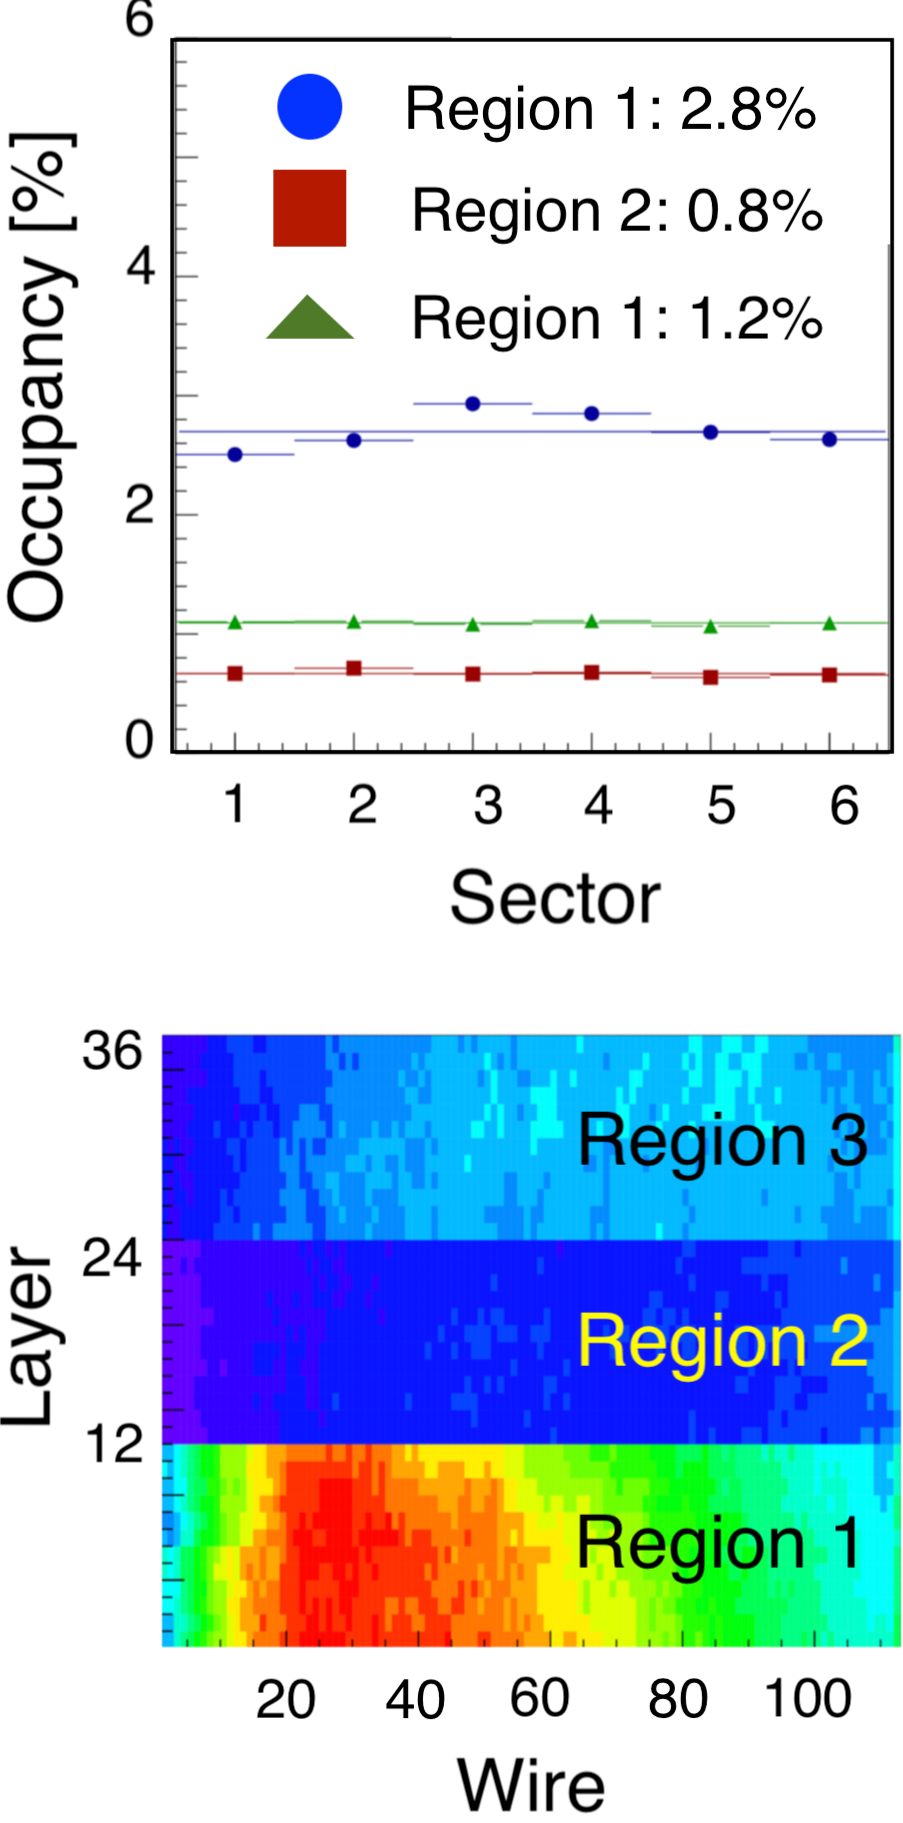
\includegraphics[width=0.99\columnwidth,keepaspectratio]{img/dcOccupancy.png}
	\caption{Results for DC rates for electron out-bending in the torus field.
		     Top: the occupancies are below $3\%$ for region 1 and below $1.2\%$ for region 3. Bottom: layer
		     versus wire hit distribution. Results for the electron in-bending polarity shows very similar distributions.}
	\label{fig:dcOccupancy}
\end{figure}

